\documentclass{beamer}

\usetheme{metropolis}

\usepackage{appendixnumberbeamer}
\usepackage{makecell}
\usepackage{graphicx}
\usepackage{makecell}
\usepackage{amsmath}
\usepackage{hyperref}
\usepackage{booktabs}
\usepackage{blkarray} % random math 
\usepackage{booktabs, multirow}
\usepackage[mathrm=sym]{unicode-math}
\usepackage{multimedia}

\setmathfont{Fira Math}
\setmathfont{Latin Modern Math}[range={\vdots,\ddots,\top}]

% --- Bibliography ---
\usepackage[authordate, backend=biber, ibidtracker=false]{biblatex-chicago} % packages
\bibliography{../paper/sources} % .bib file
\setbeamertemplate{bibliography item}{}


% --- Commands ---
\newcommand{\Var}{\mathrm{Var}}
\newcommand{\Cov}{\mathrm{Cov}}

\title{A Finite Element Approach to Reaction-Diffusion Systems}
\author{Gavin Engelstad}
\date{Fall 2024}
\institute{Math 494: Partial Differential Equations}

\begin{document}

\maketitle


\begin{frame}{Big Idea}
    \centering
    I want to solve \alert{reaction-diffusion} PDEs using the \alert{finite element method}
\end{frame}

\begin{frame}{Reaction-Diffusion Equations}
    Model the concentration of compounds over time that are simultaneously \alert{reacting} with each other and \alert{diffusing} away from itself

    \[
        \partial_t u = \underbrace{\Gamma \nabla^2 u}_{\text{Diffusion}} + \underbrace{R (u)}_{\text{Reaction}}
    \]

    {\scriptsize Where:
    \begin{description}
        \item[$u$] Vector function of concentrations
        \item[$\Gamma$] Diagonal matrix of diffusion coefficients
        \item[$R$] Reaction function
    \end{description}}
\end{frame}


\section{Method}

\begin{frame}{The Weak Form}
    The reaction-diffusion equation for one compound:
    \[
        \partial_t u_n = \gamma_n \nabla^2 u_n + r_n\left(\{u_m\}_{m = 1}^N\right)
    \]

    Multiplying by $v$ and integrating gets the \alert{weak form}:
    \[
        \int_\Omega v \partial_t u_n dA = -\gamma_n \int_\Omega \nabla v \cdot \nabla u_n dA + \int_\Omega v r_n\left(\{u_m\}_{m = 1}^N\right) dA
    \]

    \begin{center}
        \emph{I approximate the weak form of the PDE}
    \end{center}
\end{frame}

\begin{frame}{Triangulation}
    I approximate $u$ at the vertices of a \alert{triangulation} of $\Omega$
    \begin{center}
        \includegraphics{figures/tris.pdf}
    \end{center}
\end{frame}

\begin{frame}{Spacial Discretization (1/2)}
    \begin{columns}
        \begin{column}{0.4\textwidth}
            Define a function $\psi_i$ at each vertex $v_i$ that's linear on each triangle and
            \begin{align*}
                \psi_i(v_i) &= 1 \quad \\
                \quad \psi_i (v_j) &= 0
            \end{align*}
        \end{column}

        \begin{column}{0.6\textwidth}
            \centering
            \includegraphics{figures/psi.pdf}
        \end{column}
    \end{columns}
\end{frame}

\begin{frame}{Spacial Discretization (2/2)}
    Define
    \[
        \hat{u}_n (t, x, y) = \sum_i \psi_i (x, y) u_{n, i} (t) \approx u_n (t, x, y)
    \]
    \[
        \hat{r}_n (t, x, y) = \sum_i \psi_i (x, y) r_n \left(\{u_{m, i}(t)\}_{m = 1}^N\right) \approx r_n \left(\{u_m(t, x, y)\}_{m = 1}^N\right)
    \]

    Discretized weak form is
    \[
        \sum_j \partial_t u_{n, j} d_{i,j}  = -\gamma_n \sum_j u_{n, j} s_{i,j} + \sum_j r_n \left(\{u_{m, j}\}_{m = 1}^N\right) d_{i,j}
    \]
    where
    \[
        d_{i,j} = \int_\Omega \psi_i \psi_j dA \quad \text{and} \quad s_{i,j} = \int_\Omega \nabla \psi_i \cdot \nabla \psi_j dA
    \]
\end{frame}

\begin{frame}{Temporal Discretization}
    I combine an \alert{explicit} (forwards) and \alert{implicit} (backwards) Euler method

    \[
        \resizebox{\textwidth}{!}{%
        $\displaystyle \sum_j \frac{u_{n, j} (t + \Delta t) - u_{n, j} (t)}{\Delta t} d_{i,j} = \underbrace{-\gamma_n \sum_j u_{n, j} (t + \Delta t) s_{i,j}}_{\text{Implicit}} + \underbrace{\sum_j r_n \left(\{u_{m, j} (t)\}_{m = 1}^N\right) d_{i,j}}_{\text{Explicit}}$%
        }
    \]
\end{frame}

\begin{frame}{Linear System}
    Altogether, I solve for $u_n^{t + \Delta t}$ using the linear system
    \[
        (D + \Delta t \gamma_n S) u_n^{t + \Delta t} = D \left(u_n^t + \Delta t r_n \left(\{u_m^t\}_{m = 1}^N\right)\right)
    \]
    {\scriptsize
    Where
    \begin{description}
        \item[$u_n^t$] The vector of $u$ values at the vertices at time $t$
        \item[$D$] ``Damping Matrix'' of $d_{i,j}$ values
        \item[$S$] ``Stiffness Matrix'' of $s_{i,j}$ values
    \end{description}
    }
\end{frame}


\section{Solutions}

\begin{frame}{The Equation}
    As an example reaction-diffusion equation, I use
    \begin{align*}
        \frac{\partial u}{\partial t} &= \gamma_u \nabla^2 u + k_1 \left(v - \frac{uv}{1 + v^2}\right) \\
        \frac{\partial v}{\partial t} &= \gamma_v \nabla^2 v + k_2 - v - \frac{4 u v}{1 + v^2}
    \end{align*}
    with $\gamma_u = 1$, $\gamma_v = 0.02$, $k_1 = 9$, $k_2 = 11$
\end{frame}

\begin{frame}{Solution (Square)}
    \centering
    \includegraphics{figures/square.pdf}
\end{frame}

\begin{frame}{Solution (Circle)}
    \centering
    \includegraphics{figures/circle.pdf}
\end{frame}

\begin{frame}{Solution (Maze)}
    \centering
    \includegraphics{figures/maze.pdf}
\end{frame}

\begin{frame}{Solution (Sphere)}
    \centering
    \includegraphics{figures/sphere.pdf}
\end{frame}

\begin{frame}{Solution (Torus)}
    \centering
    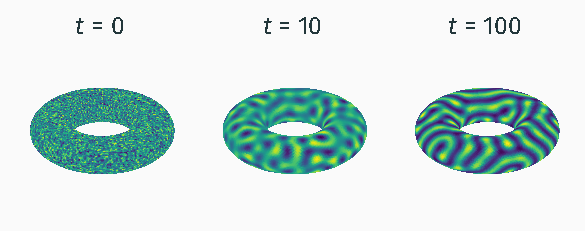
\includegraphics{figures/torus.pdf}
\end{frame}


\section{Conclusion}

\begin{frame}{Conclusion}
    I used a finite element approach to numerically solve reaction-diffusion PDEs

    Potential next steps:
    \begin{itemize}
        \item More accurate solutions
        \begin{itemize}
            \item Spectral element method
            \item Account for curvature
        \end{itemize}
        \item More realistic solutions
        \begin{itemize}
            \item The effects of tissue growth 
            \item Realistic reaction functions
        \end{itemize}
    \end{itemize}
\end{frame}

\begin{frame}[standout]
    Questions?
\end{frame}


\end{document}
